\documentclass{standalone}
\usepackage{tikz}
\usepackage{ctex,siunitx}
\usepackage{tkz-euclide}
\usepackage{amsmath}
\usetikzlibrary{patterns, calc}
\usetikzlibrary {decorations.pathmorphing, decorations.pathreplacing, decorations.shapes,}
\begin{document}
\small
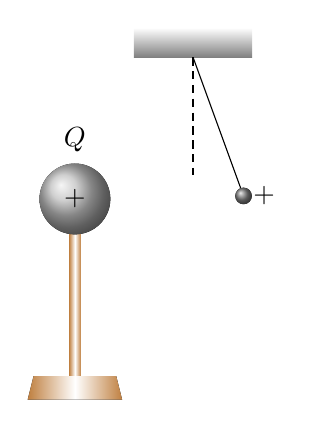
\begin{tikzpicture}[>=latex,scale=1.5]
  % \useasboundingbox(-1,-2)rectangle(8,6);
  \fill[left color=brown,right color=brown, middle color=white](-0.05,0)rectangle(0.05,-1.5);
  \fill[ball color=lightgray](0,0)circle(0.3)node{$+$};
  \node at(0,0.5){$Q$};
  \fill[left color=brown,right color=brown, middle color=white](-0.4,-1.7)--(-0.35,-1.5)--(0.35,-1.5)--(0.4,-1.7)--cycle;
  \begin{scope}[xshift=1cm,yshift=1.2cm]
    \fill[top color=white,bottom color=gray](-0.5,0)rectangle(0.5,0.25);
    \draw[thin,densely dashed](0,0)--(0,-1);
    \draw(0,0)--(-70:1.25);
    \fill[ball color=gray](-70:1.25)circle(2pt)node[right]{$+$};
  \end{scope}
\end{tikzpicture}
\end{document}